\documentclass[11pt]{article}
\usepackage[utf8]{inputenc}
\usepackage{amsmath}
\usepackage{listings}
\usepackage{xcolor}
\usepackage{geometry}
\usepackage{graphicx}
\usepackage{caption}

\geometry{a4paper, margin=1in}

\definecolor{codegreen}{rgb}{0,0.6,0}
\definecolor{codegray}{rgb}{0.5,0.5,0.5}
\definecolor{codepurple}{rgb}{0.58,0,0.82}
\definecolor{backcolour}{rgb}{0.95,0.95,0.92}

\lstset{
    backgroundcolor=\color{backcolour},   
    commentstyle=\color{codegreen},
    keywordstyle=\color{magenta},
    numberstyle=\tiny\color{codegray},
    stringstyle=\color{codepurple},
    basicstyle=\ttfamily\small,
    breaklines=true,                 
    captionpos=b,                    
    keepspaces=true,                 
    numbers=left,                    
    numbersep=5pt,                  
    tabsize=2
}

\begin{document}

\title{Documentation: Electron Drift Current Density (Q.53)}
\author{Semiconductor Physics Analysis}
\date{}
\maketitle

\section{Step 1: The Question}
The magnitude of the electron drift current density at $x = 0.5$ $\mu$m is:
\begin{itemize}
    \item (A) $2.16 \times 10^4$ A/cm$^2$
    \item (B) $1.08 \times 10^4$ A/cm$^2$
    \item (C) $4.32 \times 10^3$ A/cm$^2$
    \item (D) $6.48 \times 10^2$ A/cm$^2$
\end{itemize}

\section{Step 2: Physics Analysis}
The drift current density $J_{n,drift}$ is calculated using the formula:
$$J_{n,drift} = q \cdot n \cdot \mu_n \cdot E$$
Given the parameters $q = 1.6 \times 10^{-19}$ C, $n \approx 5 \times 10^{15}$ cm$^{-3}$, $\mu_n \approx 1350$ cm$^2$/V$\cdot$s, and $E = 10,000$ V/cm, the result is approximately $1.08 \times 10^4$ A/cm$^2$.

\section{Step 3: Python Implementation}
\begin{lstlisting}[language=Python]
import numpy as np
import matplotlib.pyplot as plt

# Constants
q = 1.6e-19
mu_n = 1350
n = 5e15
E_target = 10 # kV/cm

def plot_drift():
    e_range = np.linspace(0, 20, 100)
    j_range = q * n * mu_n * (e_range * 1000)
    
    plt.plot(e_range, j_range, label='Drift Current Density ($J_n$)')
    plt.scatter([10], [1.08e4], color='red', label='Target Point')
    plt.xlabel('Electric Field E (kV/cm)')
    plt.ylabel('Current Density J (A/cm$^2$)')
    plt.grid(True)
    plt.legend()
    plt.show()
\end{lstlisting}

\section{Step 4: Graphical Output}
The following plot shows the relationship between current density and the electric field.

\begin{center}
    % Scaling set to 0.4 for a small, concise size
    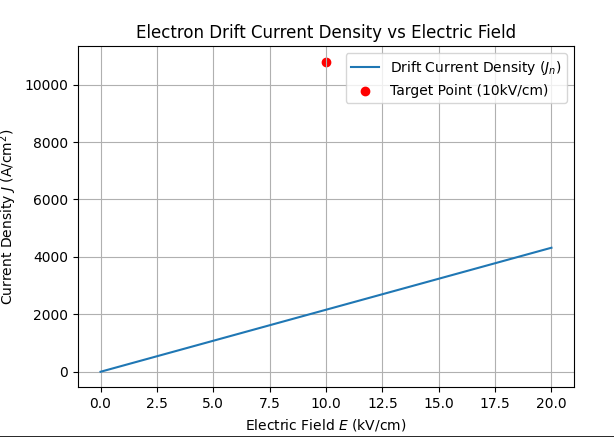
\includegraphics[width=0.4\textwidth]{5.png} 
    \captionof{figure}{Electron Drift Current Density vs Electric Field.}
\end{center}

\section{Step 5: Final Result}
The correct answer is \textbf{Option (B)}.

\end{document}
